\documentclass{beamer}
% imprimir
% \documentclass[handout]{beamer} 
% \usepackage{pgfpages}
% \pgfpagesuselayout{4 on 1}[a4paper,landscape,border shrink=5mm]

\mode<presentation> {
  \usetheme{Warsaw}
  \setbeamercovered{transparent}
}

\usebackgroundtemplate{
\includegraphics[width=\paperwidth]{format/libresoft-bg.png}}
\usepackage[spanish]{babel}
\usepackage[utf8]{inputenc}
\usepackage{graphics}
\usepackage{amssymb} % Simbolos matematicos

%\definecolor{libresoftgreen}{RGB}{162,190,43}
%\definecolor{libresoftblue}{RGB}{0,98,143}

%\setbeamercolor{titlelike}{bg=libresoftgreen}

%% Metadatos del PDF.
\hypersetup{  
  pdftitle={Tareas esenciales en la administración de sistemas},
  pdfauthor={Miguel Vidal},
  pdfcreator={GSyC/Libresoft},
  pdfproducer=PDFLaTeX,
  pdfsubject={Curso arquitectura de servidores con software libre},
}
%%

\begin{document}

\title{Tareas esenciales en la administración de sistemas}
\subtitle{Arquitectura de servidores con software libre}
\institute{\{mvidal,jfcastro\}@gsyc.urjc.es} 
\author{Miguel Vidal, José Castro}
%\date{\today}
\date{25 de marzo de 2011}

\frame{
\maketitle
\begin{center}

\includegraphics[width=6cm]{format/gsyc-urjc}
\end{center}
}

\frame{
~
\vspace{4cm}

\begin{flushright}
{\small
(cc) 2009-2011 Miguel Vidal, José Castro. \\
  Esta presentación se publica bajo una licencia Creative Commons Reconocimiento 3.0 España, disponible en 
  \url{http://creativecommons.org/licenses/by/3.0/es/}
 

\bigskip

}
\end{flushright}
}
%%

\begin{frame}
  \frametitle{Agenda}

%  \begin{itemize}[<+->]
\begin{enumerate}
\item ¿Qué es un administrador de sistemas? 
\item Deberes de un sysadmin. Cultura (\textsc{bofh}, Usenet\dots)
\item Políticas y procedimientos
\item Sistemas de seguimiento de incidencias
\item Asociaciones y organizaciones profesionales, certificaciones     
\end{enumerate}

\end{frame}

%%%%%%%%%%%%%%%%%%%%%%%%%%%%%%%%%%%%%%%%%%%%%%%%%%%%%%%%%%%%%%%%%%%%%%%
\section{¿Qué es un administrador de sistemas?}
%%%%%%%%%%%%%%%%%%%%%%%%%%%%%%%%%%%%%%%%%%%%%%%%%%%%%%%%%%%%%%%%%%%%%%%

\begin{frame}

\begin{center}
\huge{¿Qué es un administrador de sistemas?}
\end{center}

\end{frame}


%%%%%%%%%%%%%%%%%%%%%%%%%%%%%%%%%%%%%%%%%%%%%%%%%%%%%%%%%%%%%%%%%%%%%%%

\begin{frame}
\frametitle{¿Qué es un administrador de sistemas?}

``\textit{Un administrador de sistemas es aquel profesional que tiene la responsabilidad de ejecutar, mantener, operar y asegurar el correcto funcionamiento de un sistema informático y/o una red de ordenadores.}'' (Wikipedia).

\bigskip

Tambien llamado \alert{sysadmin}, debe demostrar una mezcla de \alert{cualidades técnicas} y de \alert{responsabilidad} para desempeñar bien su trabajo. 

\end{frame}

%%%%%%%%%%%%%%%%%%%%%%%%%%%%%%%%%%%%%%%%%%%%%%%%%%%%%%%%%%%%%%%%%%%%%%%

\begin{frame}
\frametitle{Tareas esenciales de la administración de sistemas}

\begin{itemize}
\item Istalación, soporte y mantenimiento de servidores o de otros sistemas informáticos.
\item \textit{Scripting} o programación ligera. 
\item Gestión de proyectos en proyectos relacionados con sistemas. 
\item Supervisión y formación de operadores. 
\item mantenimiento: Monitorización del sistema, ejecutar backups, actualizar software, añadir y retirar hardware...
\item Creación, organización y mantenimiento de la documentación.
\item Soporte a usuarios.
\end{itemize}

\small

Todas estas tareas no necesariamente las lleva a cabo una sola persona. Pero al menos una persona debe conocerlas y asegurarse de que alguien las hace.

\end{frame}


%%%%%%%%%%%%%%%%%%%%%%%%%%%%%%%%%%%%%%%%%%%%%%%%%%%%%%%%%%%%%%%%%%%%%%%

\begin{frame}
\frametitle{Habilidades}

\begin{itemize}
\item Tenacidad para resolver problemas (incluso obsesivos).
\item Deseo genuino de ayudar a la gente.
\item Los sysadmins suelen considerar divertido lo que hacen.
\end{itemize}
\end{frame}

%%%%%%%%%%%%%%%%%%%%%%%%%%%%%%%%%%%%%%%%%%%%%%%%%%%%%%%%%%%%%%%%%%%%%%%

\begin{frame}
\frametitle{Habilidades, formación}

\begin{itemize}
\item La administración de sistemas implica más cambios de contextos en un solo día que la mayoría de trabajos en un año.
\item Un sysadmin necesita habilidad para organizarse y gestionar su tiempo eficientemente.
\item Habilidad para mantener felices a los usuarios en una situación \textit{win-win}.
\item El ``queme'' en el trabajo de un sysadmins es creciente. La mayoría de los administradores duran solo unos cuantos años.
\item A diferencia de otras profesiones, no existe una única vía para convertirse en sysadmin.
\end{itemize}
\end{frame}

%%%%%%%%%%%%%%%%%%%%%%%%%%%%%%%%%%%%%%%%%%%%%%%%%%%%%%%%%%%%%%%%%%%%%%%

\begin{frame}
\frametitle{Tipos de sysadmin}

\begin{itemize}
\item senior
\item operador
\item soporte técnico 
\item administrador de base de datos (DBA)
\item administrador de seguridad
\item administrador web
\end{itemize}
\end{frame}



%%%%%%%%%%%%%%%%%%%%%%%%%%%%%%%%%%%%%%%%%%%%%%%%%%%%%%%%%%%%%%%%%%%%%%%
% \section{Duties of a system administrator}
%%%%%%%%%%%%%%%%%%%%%%%%%%%%%%%%%%%%%%%%%%%%%%%%%%%%%%%%%%%%%%%%%%%%%%%




%%%%%%%%%%%%%%%%%%%%%%%%%%%%%%%%%%%%%%%%%%%%%%%%%%%%%%%%%%%%%%%%%%%%%%%
\section{Políticas y procedimientos}
%%%%%%%%%%%%%%%%%%%%%%%%%%%%%%%%%%%%%%%%%%%%%%%%%%%%%%%%%%%%%%%%%%%%%%%


\begin{frame}

\begin{center}
\huge{Políticas y procedimientos}
\end{center}

\end{frame}

%%%%%%%%%%%%%%%%%%%%%%%%%%%%%%%%%%%%%%%%%%%%%%%%%%%%%%%%%%%%%%%%%%%%%%%

\begin{frame}
\frametitle{Documentación}

\begin{itemize}
\item Páginas \texttt{man}: tradicional doc. online.
	\begin{itemize}
	\item Están organizadas por secciones. 
	\item Una misma orden puede estar en varias secciones.
	\item No son howtos. 
	\end{itemize}
\item GNU Texinfo (Linux)
\item Guías y documentación específica de cada sistema (ej. \textit{FreeBSD Handbook} o \texttt{docs.sun.com})
\item Documentación específica del paquete: (ej. \texttt{/usr/share/doc})
\item Libros en papel (O'Reilly)
\item Linux Documentation Project
\item RFCs
\end{itemize}

\end{frame}


%%%%%%%%%%%%%%%%%%%%%%%%%%%%%%%%%%%%%%%%%%%%%%%%%%%%%%%%%%%%%%%%%%%%%%%

\begin{frame}
\frametitle{Importancia de documentar}

\begin{itemize}
\item La documentación ayuda a la reproducibilidad. 
\item La documentación ahorra tiempo. 
\item La documentación reduce la propabilidad de puntos únicos de fallo (SPoF).
\item Lo principal: la documentación mejora la inteligibilidad de un sistema y permite que
	las modificaciones se hagan de un modo consistente.
\item Escribe documentos cortos: de una página que cubran un solo tema.
\item La documentación local debe guardarse en un solo punto bien definido (wiki, repo...).
\end{itemize}

\end{frame}


%%%%%%%%%%%%%%%%%%%%%%%%%%%%%%%%%%%%%%%%%%%%%%%%%%%%%%%%%%%%%%%%%%%%%%%


%%%%%%%%%%%%%%%%%%%%%%%%%%%%%%%%%%%%%%%%%%%%%%%%%%%%%%%%%%%%%%%%%%%%%%%

\begin{frame}
\frametitle{Procedimientos}

Algunas tareas comunes que suelen necesitar procedimientos:

\begin{itemize}
\item Añadir un \textit{host}
\item Añadir un usuario
\item Configurar los backups para una nueva máquina
\item Securizar una nueva máquina
\item Actualizar el sistema operativo
\item Hacer respaldo y restauración de datos
\item Ejecutar apagados de emergencia
\end{itemize}
\end{frame}

%%%%%%%%%%%%%%%%%%%%%%%%%%%%%%%%%%%%%%%%%%%%%%%%%%%%%%%%%%%%%%%%%%%%%%%

\begin{frame}
\frametitle{Políticas}

Políticas habituales:

\begin{itemize}
\item Políticas de seguridad
\item Políticas para los administradores (login, sudo, pfexec...)
\item Acceso y políticas de usuario
\item Política de privacidad
\item Cuestiones legales: copyright (licencias y datos almacenados), cifrado, protección de datos personales\dots
\end{itemize}
\end{frame}


%%%%%%%%%%%%%%%%%%%%%%%%%%%%%%%%%%%%%%%%%%%%%%%%%%%%%%%%%%%%%%%%%%%%%%%
\section{Sistemas de seguimiento de incidencias}
%%%%%%%%%%%%%%%%%%%%%%%%%%%%%%%%%%%%%%%%%%%%%%%%%%%%%%%%%%%%%%%%%%%%%%%


\begin{frame}
\frametitle{Sistemas de seguimiento de incidencias}

\begin{itemize}
\item Software para crear, actualizar y resolver listas de incidencias. Similar a una 
"bugtracker". 
\item Contiene una base de conocimientos con soluciones a problemas comunes: recurso de valor incalculable para el personal administrador de sistemas. 
\item \alert{Ticket/incidencia:} una ficha que contiene información sobre las intervenciones de soporte realizadas por el personal técnico. 
\item Trac (python), RT (Perl), Redmine (RoR), OTRS, Mantis...: \url{http://en.wikipedia.org/wiki/Comparison_of_issue_tracking_systems}
\end{itemize}
\end{frame}

%%%%%%%%%%%%%%%%%%%%%%%%%%%%%%%%%%%%%%%%%%%%%%%%%%%%%%%%%%%%%%%%%%%%%%%


\begin{frame}
\frametitle{Funciones comunes de un sistema de gestión de incidencias}

Los responsables de proyecto pueden extraer valiosa información de alto nivel como:

\begin{itemize}
\item El número de tickets abiertos 
\item El tiempo medio en cerrarse un ticket
\item La productividad de los sysadmins
\item El porcentaje de tickets no resueltos
\item Posibles desequilibrios en la distribución de la carga de trabajo

\end{itemize}
\end{frame}


%%%%%%%%%%%%%%%%%%%%%%%%%%%%%%%%%%%%%%%%%%%%%%%%%%%%%%%%%%%%%%%%%%%%%%%

\begin{frame}
\frametitle{Flujo}

\begin{itemize}
\item El usuario (o el \textit{helpdesk}) reporta un problema.
\item El operador verifica que el problema es real y no solo una impresión.
\item EL operador se asegura de obtener suficiente información sobre el problema por parte del usuario.
\item La incidencia se asigna a la persona adecuada, que la marca como resuelta/cerrada/wontfix/feedback

\end{itemize}
\end{frame}

%%%%%%%%%%%%%%%%%%%%%%%%%%%%%%%%%%%%%%%%%%%%%%%%%%%%%%%%%%%%%%%%%%%%%%%

\begin{frame}
\frametitle{Redmine}

Principales características:
\begin{itemize}
\item Soporte multi-proyecto
\item ACLs: acceso basado en roles muy flexibles. 
\item Wiki por proyecto
\item Integración con SCM (SVN, CVS, Git, Mercurial, Bazaar y Darcs)
\item Soporte para auto-registro
\item Diagrama de Gantt y calendario
\item Feeds y notificación por e-mail.
\end{itemize}
\end{frame}


%%%%%%%%%%%%%%%%%%%%%%%%%%%%%%%%%%%%%%%%%%%%%%%%%%%%%%%%%%%%%%%%%%%%%%%

\begin{frame}
\frametitle{Certificación UNIX}

\begin{itemize}
\item \textsc{UNIX}\texttrademark{} es una marca registrada propiedad del Open Group consortium (Fujitsu, Sun, Hitachi, HP, IBM, NEC, US DoD, la NASA y otros). 
\item Open Group se encarga de conceder certificados SUS: Single UNIX Specification 
\item Solaris, HP-UX, AIX y MacOS X tienen certificación SUS
\item Tipo Unix (\textit{Unix-like}): Linux, BSD y OpenSolaris
\end{itemize}
\end{frame}


%%%%%%%%%%%%%%%%%%%%%%%%%%%%%%%%%%%%%%%%%%%%%%%%%%%%%%%%%%%%%%%%%%%%%%%

\begin{frame}
\frametitle{Timeline de Unix}
\begin{center}
  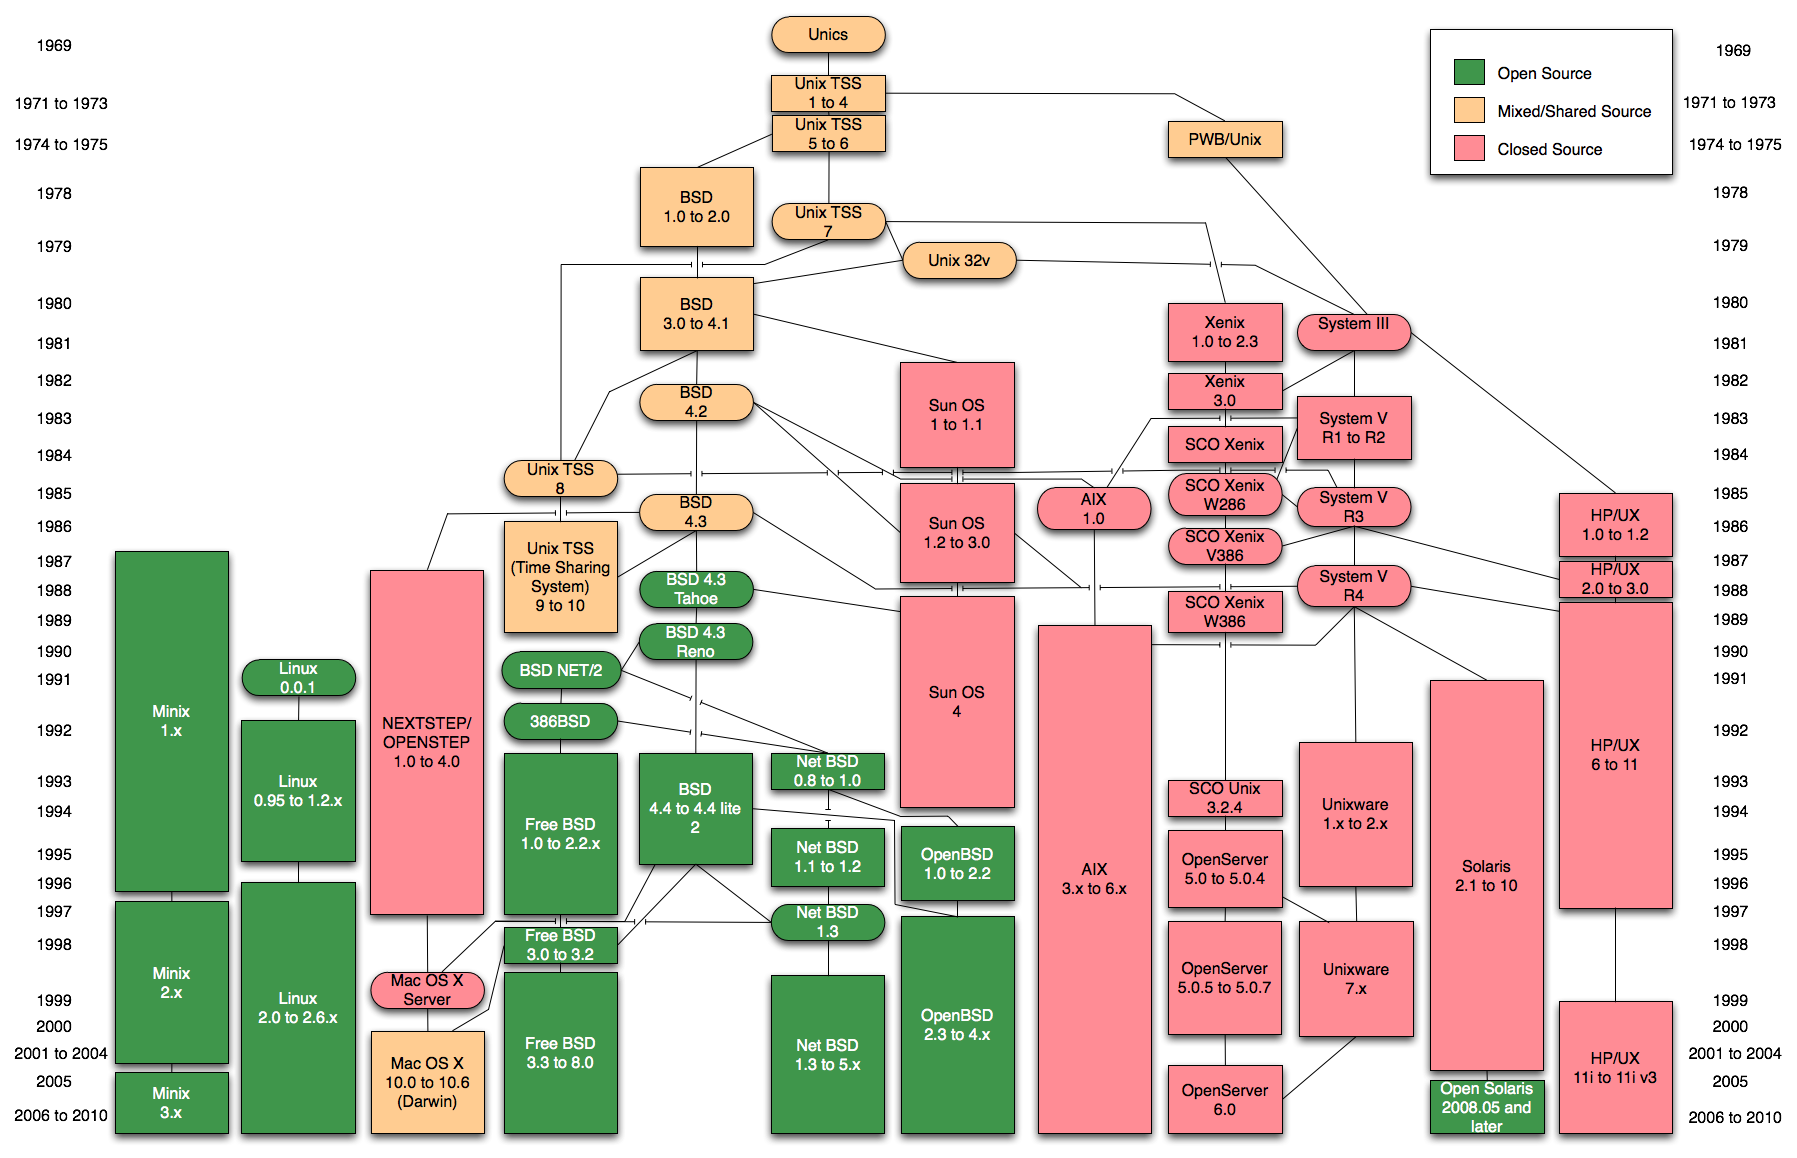
\includegraphics[height=2.5in]{figs/Unix_history-simple.png}
\end{center}
\end{frame}

%%%%%%%%%%%%%%%%%%%%%%%%%%%%%%%%%%%%%%%%%%%%%%%%%%%%%%%%%%%%%%%%%%%%%%%

\begin{frame}
\frametitle{Timeline de Unix}
\begin{center}
  \includegraphics[height=2.7in]{figs/2000px-Unix.png}
\end{center}
\end{frame}


%%%%%%%%%%%%%%%%%%%%%%%%%%%%%%%%%%%%%%%%%%%%%%%%%%%%%%%%%%%%%%%%%%%%%%%
\section{Asociaciones y organizaciones profesionales}
%%%%%%%%%%%%%%%%%%%%%%%%%%%%%%%%%%%%%%%%%%%%%%%%%%%%%%%%%%%%%%%%%%%%%%%

\begin{frame}

\begin{center}
\huge{Asociaciones y organizaciones profesionales}
\end{center}

\end{frame}

%%%%%%%%%%%%%%%%%%%%%%%%%%%%%%%%%%%%%%%%%%%%%%%%%%%%%%%%%%%%%%%%%%%%%%%

\begin{frame}
\frametitle{SAGE}

\begin{itemize}
\item Es la primera organización internacional para sysadmins.
\item Es un grupo de interés dentro de Usenix.
\item Promueve la admnistración de sistemas como profesión y patrocina confenrencias y programas informales.
\item Organiza el mayor evento para sysadmins: la conferencia USENIX LISA (Large Installation System Administration) en otoño.
\item SAGE se enfoca más a la investigación.
\end{itemize}
\end{frame}

%%%%%%%%%%%%%%%%%%%%%%%%%%%%%%%%%%%%%%%%%%%%%%%%%%%%%%%%%%%%%%%%%%%%%%%


\begin{frame}
\frametitle{LOPSA}

\begin{itemize}
\item LOPSA, League of Professional System Administrators.
\item Se creó en 2005 por parte de algunos miembros de SAGE. 
\item Misión: 
	\begin{itemize}
	\item promover la práctica de la administración de sistemas; 
	\item apoyar, reconocer, educar y alentar a los sysadmins; 	
 	\item servir al público por medio de la educación y divulgación en temas relacionados con la administración de sistemas.
	\end{itemize}
\item LOPSA busca brindar apoyo legislativo a los temas que afectan a la profesión.
\item SAGE y LOPSA cooperar en objetivos comunes, como el Código de Ética y la conferencia LISA.

\end{itemize}
\end{frame}

%%%%%%%%%%%%%%%%%%%%%%%%%%%%%%%%%%%%%%%%%%%%%%%%%%%%%%%%%%%%%%%%%%%%%%%

\begin{frame}
\frametitle{Herencia de Unix}

\begin{itemize}
\item ``KISS'', ``Small is beautiful'', ``Haz que cada programa haga bien una sola cosa'', ``Construye un prototipo tan pronto como sea posible'', ``Escoge la portabilidad sobre la eficiencia'', ``Usa scripts de shell scripts para incrementar la portabilidad'', ``Evita interfaces que hagan cautivos a los usuarios'', ``Haz de cada programa un filtro''...
\item Usenet, Internet jargon... 
\item System Administrator Appreciation Day (último viernes de julio)
\item Bastard Operator From Hell (BOFH)
\end{itemize}
\end{frame}


%%%%%%%%%%%%%%%%%%%%%%%%%%%%%%%%%%%%%%%%%%%%%%%%%%%%%%%%%%%%%%%%%%%%%%%

\begin{frame}
\frametitle{Código ético (1)}

LOPSA, USENIX y SAGE animan a que todo administrador se guía por un código ético:  

\begin{itemize}
\item Profesionalidad
\item Integridad personal
\item Privacidad
\item Leyes y políticas
\item Communicación
\end{itemize}
\end{frame}

%%%%%%%%%%%%%%%%%%%%%%%%%%%%%%%%%%%%%%%%%%%%%%%%%%%%%%%%%%%%%%%%%%%%%%%

\begin{frame}
\frametitle{Código ético (2)}

\begin{itemize}
\item Integridad de sistema
\item Educación
\item Responsibilidad social
\item Responsibilidad ética
\end{itemize}

\url{http://lopsa.org/CodeOfEthics}

\end{frame}

%%%%%%%%%%%%%%%%%%%%%%%%%%%%%%%%%%%%%%%%%%%%%%%%%%%%%%%%%%%%%%%%%%%%%%%

\begin{frame}
\frametitle{Referencias}

\begin{itemize}
\item Nemeth, Snyder, Hein \textit{UNIX and Linux System Administration Handbook}
\item Limoncelli, Thomas A. \textit{Time Management for System Administrators} 
\end{itemize}

\end{frame}


\end{document}




